\chapter[Mozart and Piano Sonata No. 10, K. 330]{Wolfgang Amadeus Mozart - Piano Sonata No. 10 in C major, K. 330 (1784)}\label{mozart}
Wolfgang Amadeus (W.A.) Mozart (1756-1791) was a prolific composer during the Classical period (1730-1820) of music. Mozart was born in Salzburg, in the Holy Roman Empire, on January 27, 1756\autocite{Burkholder_Grout_Palisca_2014}. He was born into a talented musical family, and by age five showed a prodigal ability in performance, specifically on the keyboard and violin \autocite{Eisen_Sadie_2001}. Mozart started performing as a court musician in the Salzburg court when he was 17, and began traveling. These travels eventually brought him to Vienna in 1781, where he chose to stay. While in Vienna, Mozart composed his \textit{Piano Sonata No. 10 in C Major}. This sonata has three movements, the allegro moderato in C Major, the Andante cantabile in F Major\footnote{This movement is in C Major's subdominant key, an important concept explained later.}, and the allegretto movement. 

The \textit{Piano Sonata in C Major} follows the standard structure of a sonata. A sonata is known to be an instrumental piece which contains one or more movements, and designed to be performed by either a soloist or a small ensemble\autocite{Mangsen_Irving_Rink_Griffiths_2014}. Each period of music had its own specific definition of a sonata, and the Classical period was no different\footnote{As stated by Mangsen et al., the definition of a sonata evolved. The definition of a sonata started generally as an instrumental piece in the thirteenth century, and was known as a \say{sonnade.} Through the development of instrumental music in the following centuries, the current definition of a sonata comes from its connotations and associations in the Classical and Romantic periods of music. The sonatas of these times were frequently assumed to be instrumental pieces in which one or more movements are incorporated. More information can be found in \citeauthor{Mangsen_Irving_Rink_Griffiths_2014} \citeyear{Mangsen_Irving_Rink_Griffiths_2014}}. Though definitions vary, generally the Classical period sonata is understood to be a musical work composed of three or four movements, most often for a piano solo \footnote{A duo between instruments such as the violin and piano were other popular choices.}. The first movement may be preceded by a slow introduction, but it is normally in sonata form. This is followed by a slow second movement, in which the key modulates to another, related key. Finally, the third movement follows as a finale, which wraps up the work.\autocite{Mangsen_Irving_Rink_Griffiths_2014} Sonata form itself is composed of three sections in a two-part tonal structure.\footnote{This two-part tonal structure is known as \say{binary form.} According to \citeauthor{Sutcliffe_Tilmouth_2001}, binary form is defined as a musical structure which consists of two sections, of roughly equal duration. This is often notated as \textit{AB}, or \textit{A$A^`$}. The form itself is characterized by the clear move to another key, followed by another clear return to the tonic key. At the end of the \textit{A} section, there is a conclusive-sounding arrival on a contrasting key (which is often the dominant key) to signify the end of the \textit{A} section. The \textit{B} section's key will then modulate to the key that was referenced at the end of the \textit{A} section. At the end of the \textit{B} section, there is a matching conclusive arrival to what we saw at the end of the \textit{A} section, this time returning to the tonic key found in the \textit{A} section. Both the \textit{A} and \textit{B} sections may also be marked by a repeat sign, to be played through twice. More information can be read in \citeauthor{Sutcliffe_Tilmouth_2001} \citeyear{Sutcliffe_Tilmouth_2001}} 

Of the three movements of the sonata form, we divide them into two tonal parts. First, there is the \say{exposition} section, which is the first in the two-part tonal structure. The exposition, as the first section in both the sonata form and the two-part tonal structure, will contain the themes through which the rest of the movement and the piece are to be based on. The exposition will open in the piece's tonic key, and concludes in a new key. This new key is typically the dominant key of the exposition section's key if the piece is in a major key\autocite{Webster_2001}--which is a fifth interval away from the key in the exposition. With the exposition conclusively arriving in a new key, the piece moves to the \say{development} section. Once the development section arrives, we have moved into the second part of the two-part tonal structure. This part of the tonal structure includes both the development and recapitulation\autocite{Webster_2001}. The development section takes the thematic material that was presented in the exposition section, and manipulates it, moving both themes and key away from the exposition.\footnote{Some of these thematic manipulations include reshaping the material on a motivic level, on a harmonic level, or on a counterpoint level, or some combination of these levels.} The ending of the development section will lead into the \say{recapitulation} section. This recapitulation section is the final section of the sonata form, and is also a part of the second section of the two-part tonal structure. It signifies the return to the tonic key of the exposition section\autocite{Webster_2001}, and restates the thematic material from that first section.

\section{Movement I: Allegro moderato}
The first movement in Mozart's \textit{Piano Sonata in C Major} is the Allegro moderato. As is typical of sonatas, this first movement is light and energetic, evidenced by Mozart's choice to use cut-time (two-four time instead of the more widely used four-four time), and the thirty-second notes instead of sixteenth-notes, like in figure \ref{fig:mozart-thirty-second-notes}\autocite{Henle_1977}. There are two main themes, or subjects, which alternate between legato and staccato. These subjects are placed over an energetic bass voice, comprised of flowing eighth and sixteenth notes.

\begin{figure}
    \centering
    \includegraphics[width=0.5\textwidth]{figures/mozart-thirty-second-notes.png}
    \caption{An example of thirty-second notes, seen in Mozart's \textit{Piano Sonata in C Major}}
    \label{fig:mozart-thirty-second-notes}
\end{figure}

\begin{figure}
    \centering
    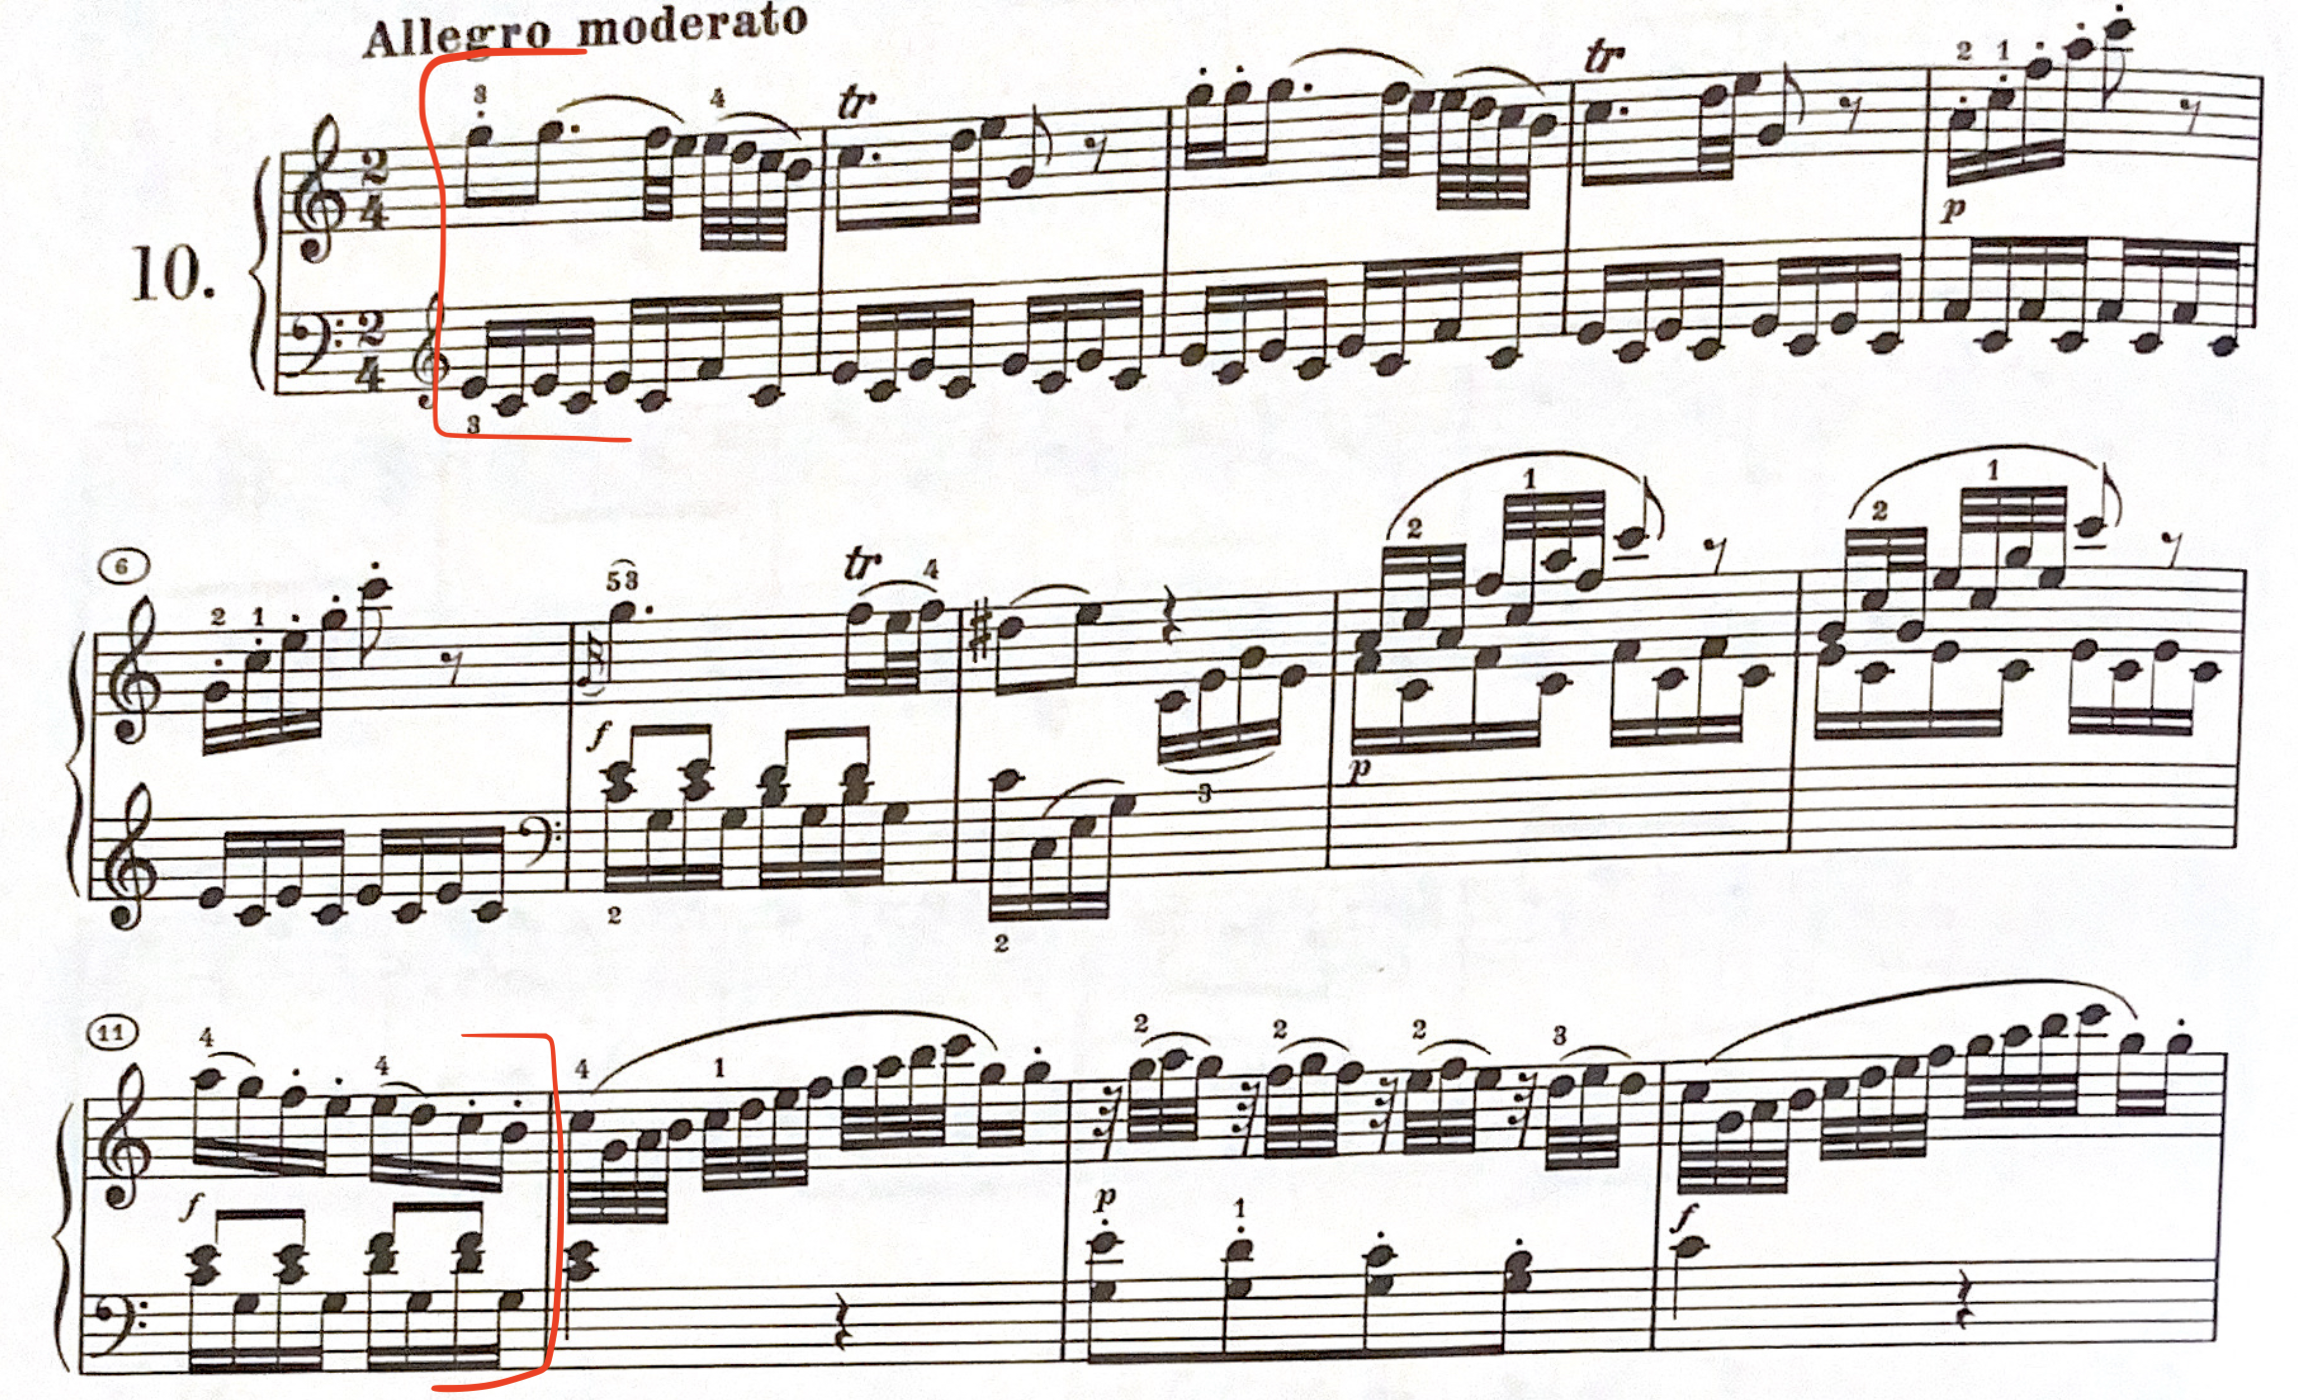
\includegraphics[width=\textwidth]{figures/mozart-first-movement-first-theme.png}
    \caption{The first of two themes seen in Mozart's \textit{Piano Sonata in C Major}}
    \label{fig:mozart-first-movement-first-theme}
\end{figure}

\begin{figure}
    \centering
    \includegraphics[width=\textwidth]{figures/mozart-first-movement-second-theme.jpg}
    \caption[The second theme in Mozart's \textit{Piano Sonata in C Major, K. 330}]{The beginning of the second of the two themes seen in Mozart's \textit{Piano Sonata in C Major}}
    \label{fig:mozart-first-movement-second-theme}
\end{figure}

The movement has two major themes, each decorated with ornamentation\footnote{This is defined as the decoration of a melodic or harmonic line in music. More reading can be found in \citeauthor{Latham_2011} \autocite{Burkholder_Grout_Palisca_2014}}. The first twelve bars of the movement begin the exposition section. Within this section, we have two themes. The first theme, as seen in figure \ref{fig:mozart-first-movement-first-theme}\autocite{Henle_1977}, lasts from bars one through twelve, and marked in red. This theme starts in the piece's tonic key of C Major. The second theme in figure \ref{fig:mozart-first-movement-second-theme}\autocite{Henle_1977} begins in bar nineteen, and is marked by a modulation to G Major, the dominant key of the piece's tonic key C Major. The exposition section sets up the primary theme of the movement as a whole. The first theme, which is seen in figure \ref{fig:mozart-first-movement-first-theme}\autocite{Henle_1977}, will be the theme through which the remainder of the movement is based on. The exposition's second theme, from figure \ref{fig:mozart-first-movement-second-theme}\autocite{Henle_1977}, is also elaborated upon later in the piece. 

There is a development section introduced in bar fifty-nine, as in figure \ref{fig:mozart-first-movement-development-start}\autocite{Henle_1977}. This section is more intense than the exposition section, with more modulations. Bar sixty-nine and bar seventy show the modulation to A Major\footnote{See figure \ref{fig:mozart-first-movement-modulation-a-major} \citeauthor{Henle_1977}}. This section also modulates to F Major\footnote{See figure \ref{fig:mozart-first-movement-f-major} \citeauthor{Henle_1977}}, D Minor\footnote{See figure \ref{fig:mozart-first-movement-d-minor} \citeauthor{Henle_1977}}, before modulating back to the tonic key of C Major for the recapitulation section. In addition to the many modulations to related keys to the tonic C Major, the development section also contains references to thematic material of the first section. The bass voice in the first theme of the exposition section, as in figure \ref{fig:mozart-first-movement-first-theme}\autocite{Henle_1977}, contains energetic sixteenth notes for the entirety of the theme. This is referred to in the development section, with bars fifty-nine to sixty-three, as in figure \ref{fig:mozart-first-movement-development-reference-first-theme}\autocite{Henle_1977}, bracketed in red. 

\begin{figure}
    \centering
    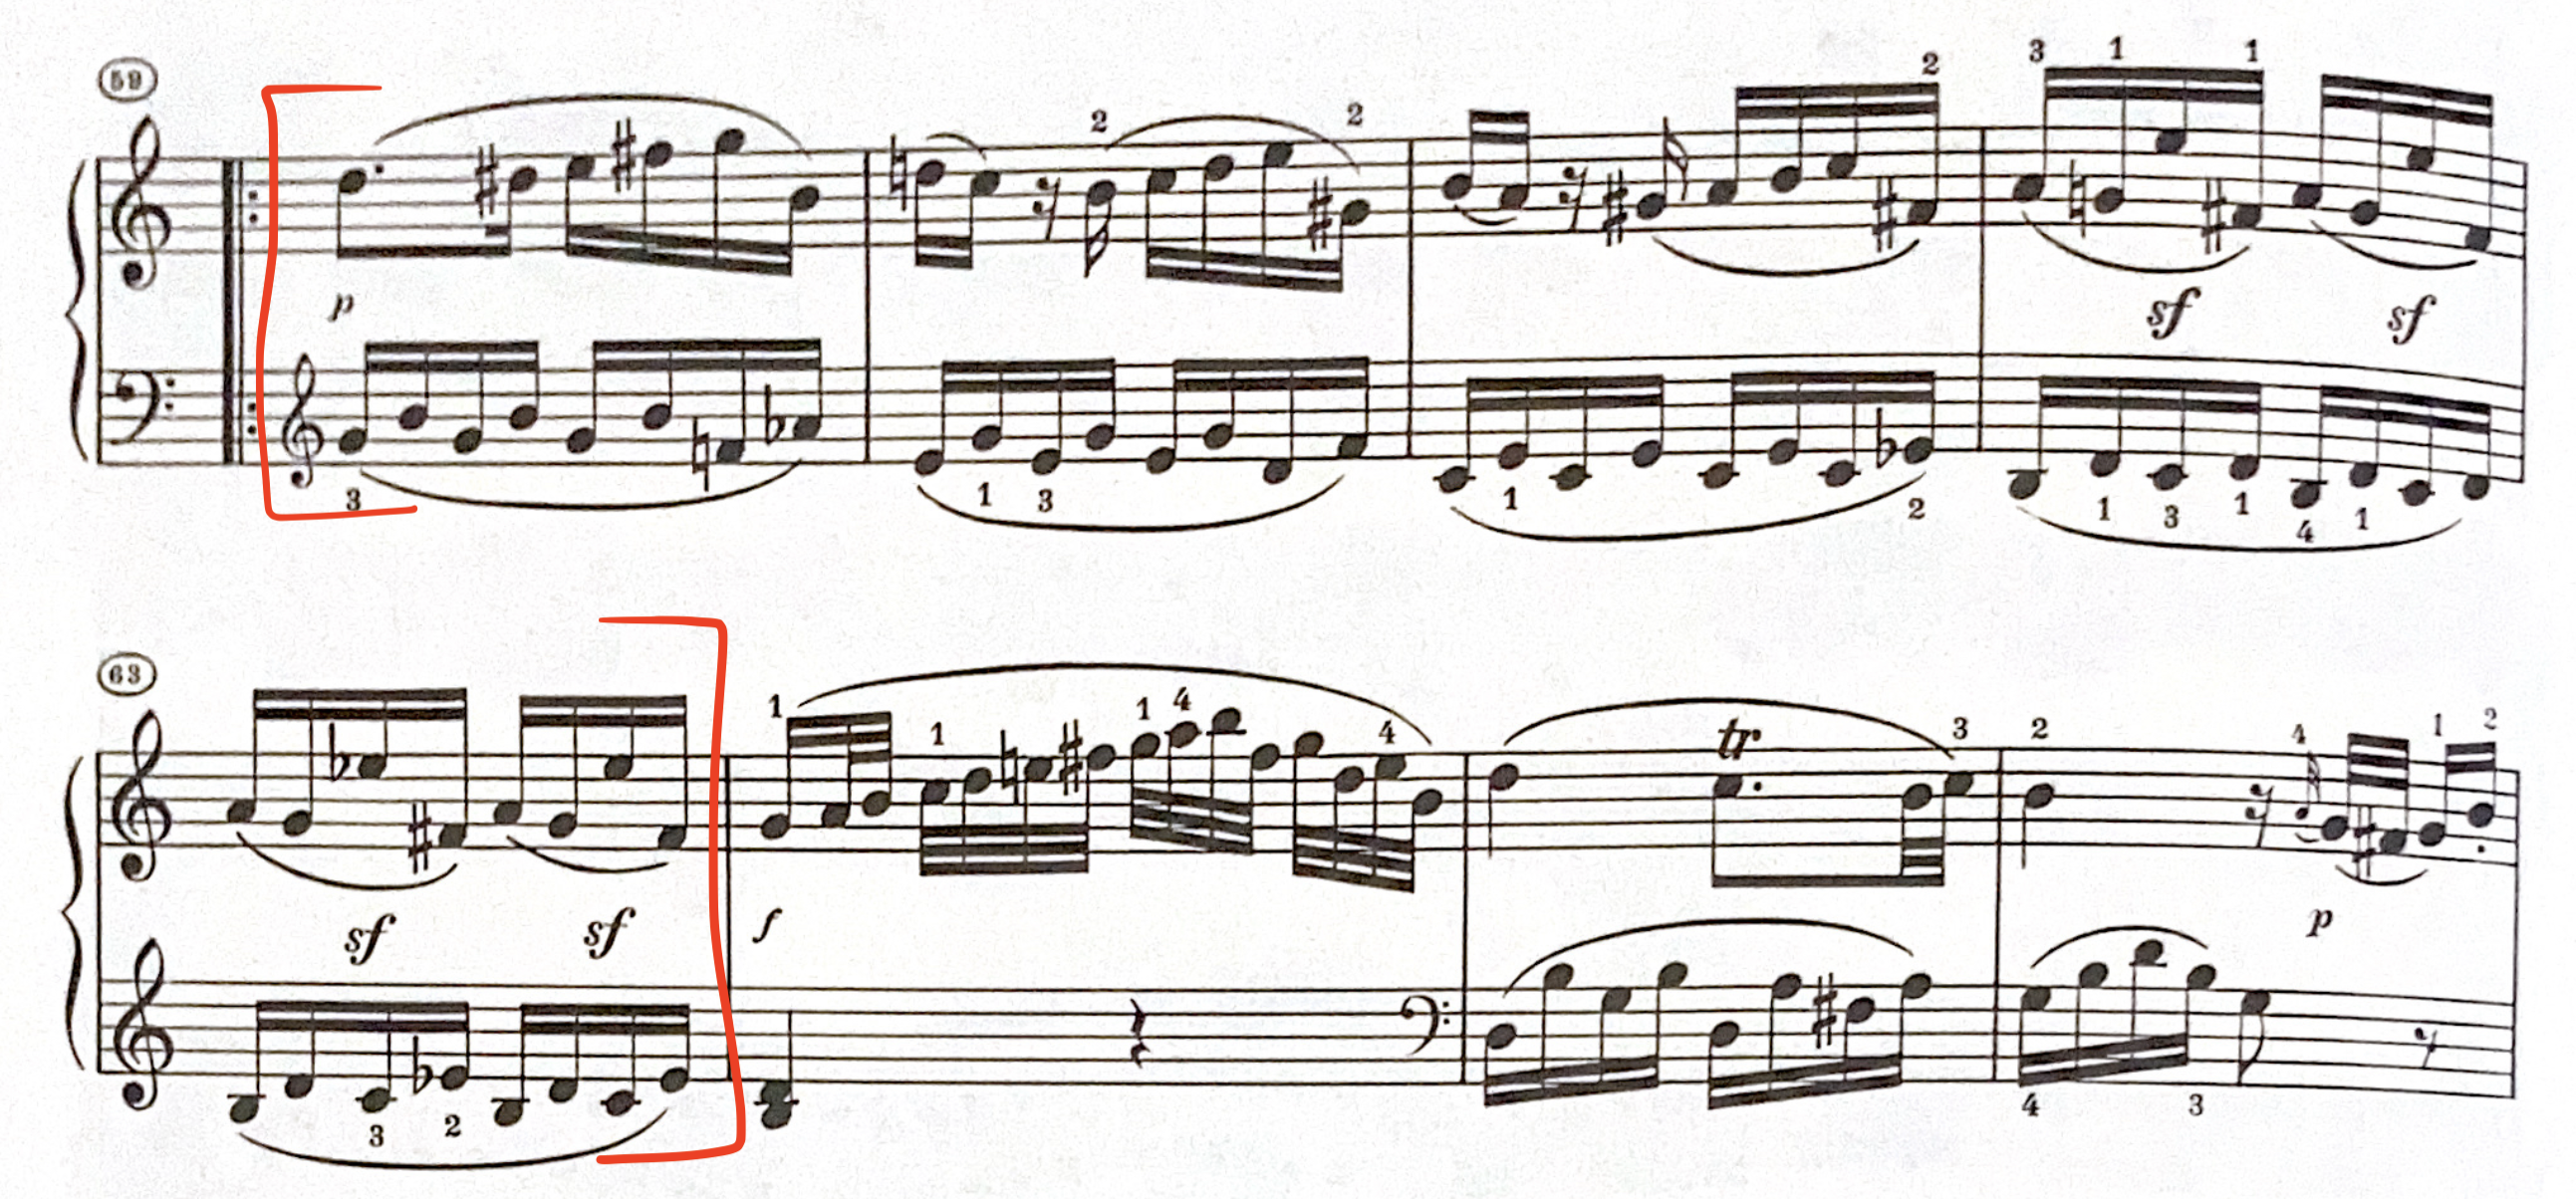
\includegraphics[width=\textwidth]{figures/mozart-first-movement-development-reference-first-theme.png}
    \caption{The reference to the first theme in the exposition section, found in the development section, in Mozart's \textit{Piano Sonata in C Major}}
    \label{fig:mozart-first-movement-development-reference-first-theme}
\end{figure}

\begin{figure}
    \centering
    \includegraphics[width=\textwidth]{figures/mozart-first-movement-development-start.png}
    \caption{The beginning of the development section in the first movement of Mozart's \textit{Piano Sonata in C Major}}\autocite{Henle_1977}
    \label{fig:mozart-first-movement-development-start}
\end{figure}

\begin{figure}
    \centering
    \includegraphics[width=0.5\textwidth]{figures/mozart-first-movement-modulation-a-major.png}
    \caption{The modulation to A Major, in Mozart's \textit{Piano Sonata in C Major}}
    \label{fig:mozart-first-movement-modulation-a-major}
\end{figure}

\begin{figure}
    \centering
    \includegraphics[width=0.5\textwidth]{figures/mozart-first-movement-f-major.png}
    \caption{The modulation to F Major, in Mozart's \textit{Piano Sonata in C Major}}
    \label{fig:mozart-first-movement-f-major}
\end{figure}

\begin{figure}
    \centering
\includegraphics[width=0.5\textwidth]{figures/mozart-first-movement-d-minor.png}
    \caption{The modulation to D Minor, in Mozart's \textit{Piano Sonata in C Major}}
    \label{fig:mozart-first-movement-d-minor}
\end{figure}

\begin{figure}
    \centering
    \includegraphics[width=\textwidth]{figures/mozart-first-movement-recapitulation-first-theme.png}
    \caption[The first theme of the exposition, found in the recapitulation, from Mozart's \textit{Piano Sonata in C Major, K. 330}]{The recapitulation section in Mozart's \textit{Piano Sonata in C Major}, where the first theme from the exposition section is heard again}
    \label{fig:mozart-first-movement-recapitulation-first-theme}
\end{figure}

Finally, in the recapitulation section, the first subject is heard again, in C Major, as in figure \ref{fig:mozart-first-movement-recapitulation-first-theme}\autocite{Henle_1977}. The recapitulation section is similar in structure to the exposition section, with the first theme in tonic key C Major, and the second theme in dominant key G Major. There are few changes made to these two themes in this section, beyond a higher amount of ornamentation added to various bars. Thus, we see that the first movement itself is also in sonata form, with an exposition section, development section, and recapitulation section.

\section{Movement II: Andante cantabile}

The second movement of Mozart's \textit{Piano Sonata in C Major}, the Andante cantabile, is marked with the modifier \say{cantabile,} meaning \say{song-like} and is reflected in the overall tonality of this movement being similar to a very sweet song. This movement is in ternary form\footnote{Ternary form is a musical structure which consists of three sections, hence the qualifier ternary. Its representation may be in the form of letter scheme ABA, with the final section A being a repetition of the first section. Each section of the ternary form is usually, but not always, self-contained and closes (or ends) in its key. The first A section will normally close in the tonic key. Then, the middle section will provide a strong contrast to the two sections which surround it, both in tone and theme.} and in the key F Major. This is important to note, as this is a modulation from the first movement, in which the key was C Major. This movement has the tonic key in F Major, whose dominant key is now C Major. The beginning 'A' section, as seen in figure \ref{fig:mozart-second-movement-first-a-section}\autocite{Henle_1977} and bracket in red, is a twenty-bar melody, broken into two sections by the repeat, and contains a repeated-note motif. The first section is comprised of the first eight bars, from the beginning up to the repeat sign\footnote{See figure \ref{fig:mozart-second-movement-first-a-section} \citeauthor{Henle_1977}}. This repeated-note motif is seen in the opening's frequent use of the note 'C' in figure \ref{fig:mozart-second-movement-first-eight-bars}\autocite{Henle_1977}\footnote{The first eight bars are bracketed in red.}. There are four repeated C's, of which the note C is imitated and repeated several times through these eight bars.

\begin{figure}
    \centering
    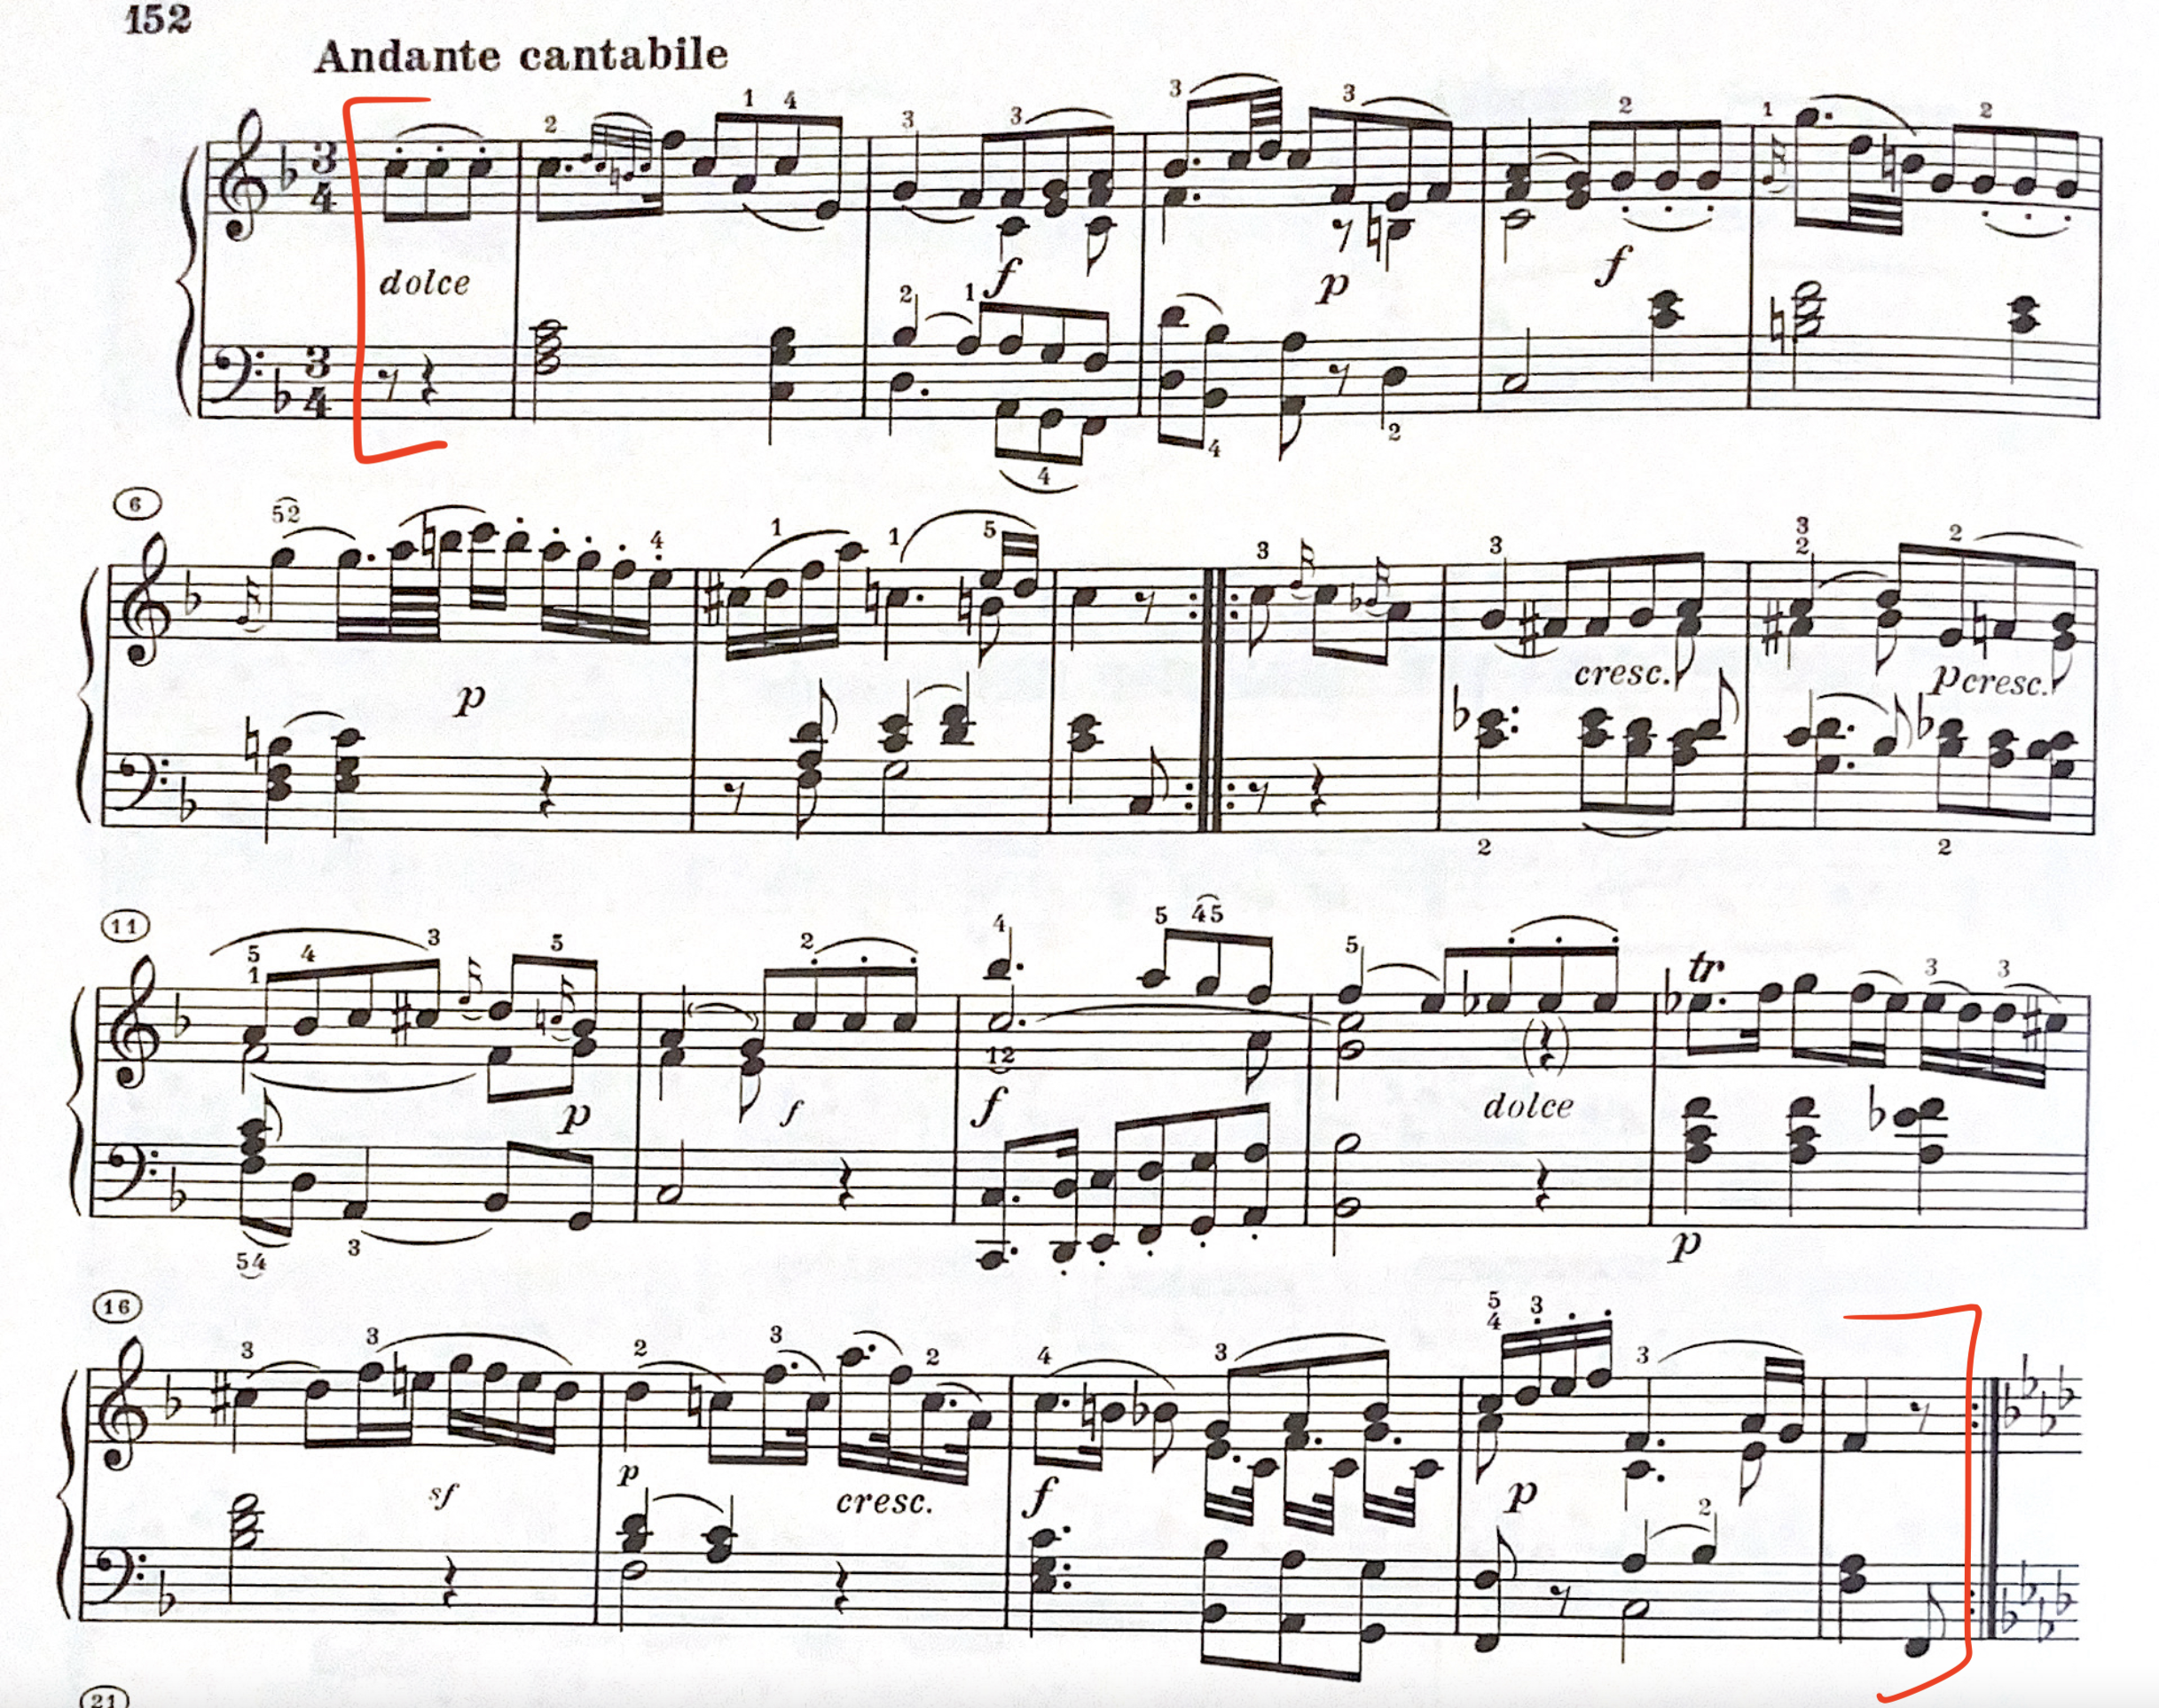
\includegraphics[width=\textwidth]{figures/mozart-second-movement-first-a-section.png}
    \caption{The first A section of the second movement of Mozart's \textit{Piano Sonata in C Major}}
    \label{fig:mozart-second-movement-first-a-section}
\end{figure}

\begin{figure}
    \centering
    \includegraphics[width=0.5\textwidth]{figures/mozart-second-movement-first-eight-bars.png}
    \caption{The first eight bars of the second movement of Mozart's \textit{Piano Sonata in C Major}}
    \label{fig:mozart-second-movement-first-eight-bars}
\end{figure}

\begin{figure}
    \centering
    \includegraphics[width=0.5\textwidth]{figures/mozart-second-movement-repeated-note-motif-middle-section.png}
    \caption{The repeated-note motif, found in the middle section of Mozart's \textit{Piano Sonata in C Major} of the second movement}
    \label{fig:mozart-second-movement-middle-section-motif}
\end{figure}

After the repetition, the middle section turns to the movement's tonic minor key\footnote{So, going from the movement's tonic key of F Major to its minor key of F Minor.}. Its melody starts in bar twenty-one, reminiscent and similar to the preceding section, with similar rhythm and usage of a repeated-note motif, as in figure \ref{fig:mozart-second-movement-middle-section-motif}\autocite{Henle_1977}. From here, it is clear to see that the first movement in of itself contains the format of a sonata form: there is an exposition, development, and recapitulation section.

\section{Movement II: Allegretto}
The third movement of Mozart's \textit{Piano Sonata in C Major}, the Allegretto, is the piece's most energetic movement. The use of arpeggios, or the sounding of a chord's notes in succession rather than in unison\autocite{Arpeggio_2001}\footnote{Arpeggios are noticeable in keyboard music, in which a chord is much more easily able to be spread out or broken apart. The keyboard is much more built for an arpeggio figuration, as each note of a chord can be played independently much easier on it.}, is prevalent throughout the movement. This movement also shares several characteristics with the first movement, including the most important: the sonata form. The third movement itself has the form of a sonata, as did the first movement, with an exposition, development, and recapitulation section. The exposition section contains a similar-sounding dotted-eighth note motif as in the first movement, as seen in figure \ref{fig:mozart-third-movement-dotted-eighth-notes-and-exposition}\autocite{Henle_1977}. The development section, on the other hand, has no relation with the material worked on within the exposition section. Its thematic material instead consists of its own figures, solely found in this section. Finally, the recapitulation features a short coda, as seen in figure \ref{fig:mozart-third-movement-coda}\autocite{Henle_1977}, and full chords. This ends the movement and the piece on a triumphant-sound, as is typical of the sonata form.

\begin{figure}
    \centering
    \includegraphics[width=\textwidth]{figures/mozart-third-movement-dotted-eighth-notes-and-exposition.png}
    \caption{The dotted-eighth note motif in the third movement of Mozart's \textit{Piano Sonata in C Major}}
    \label{fig:mozart-third-movement-dotted-eighth-notes-and-exposition}
\end{figure}

\begin{figure}
    \centering
    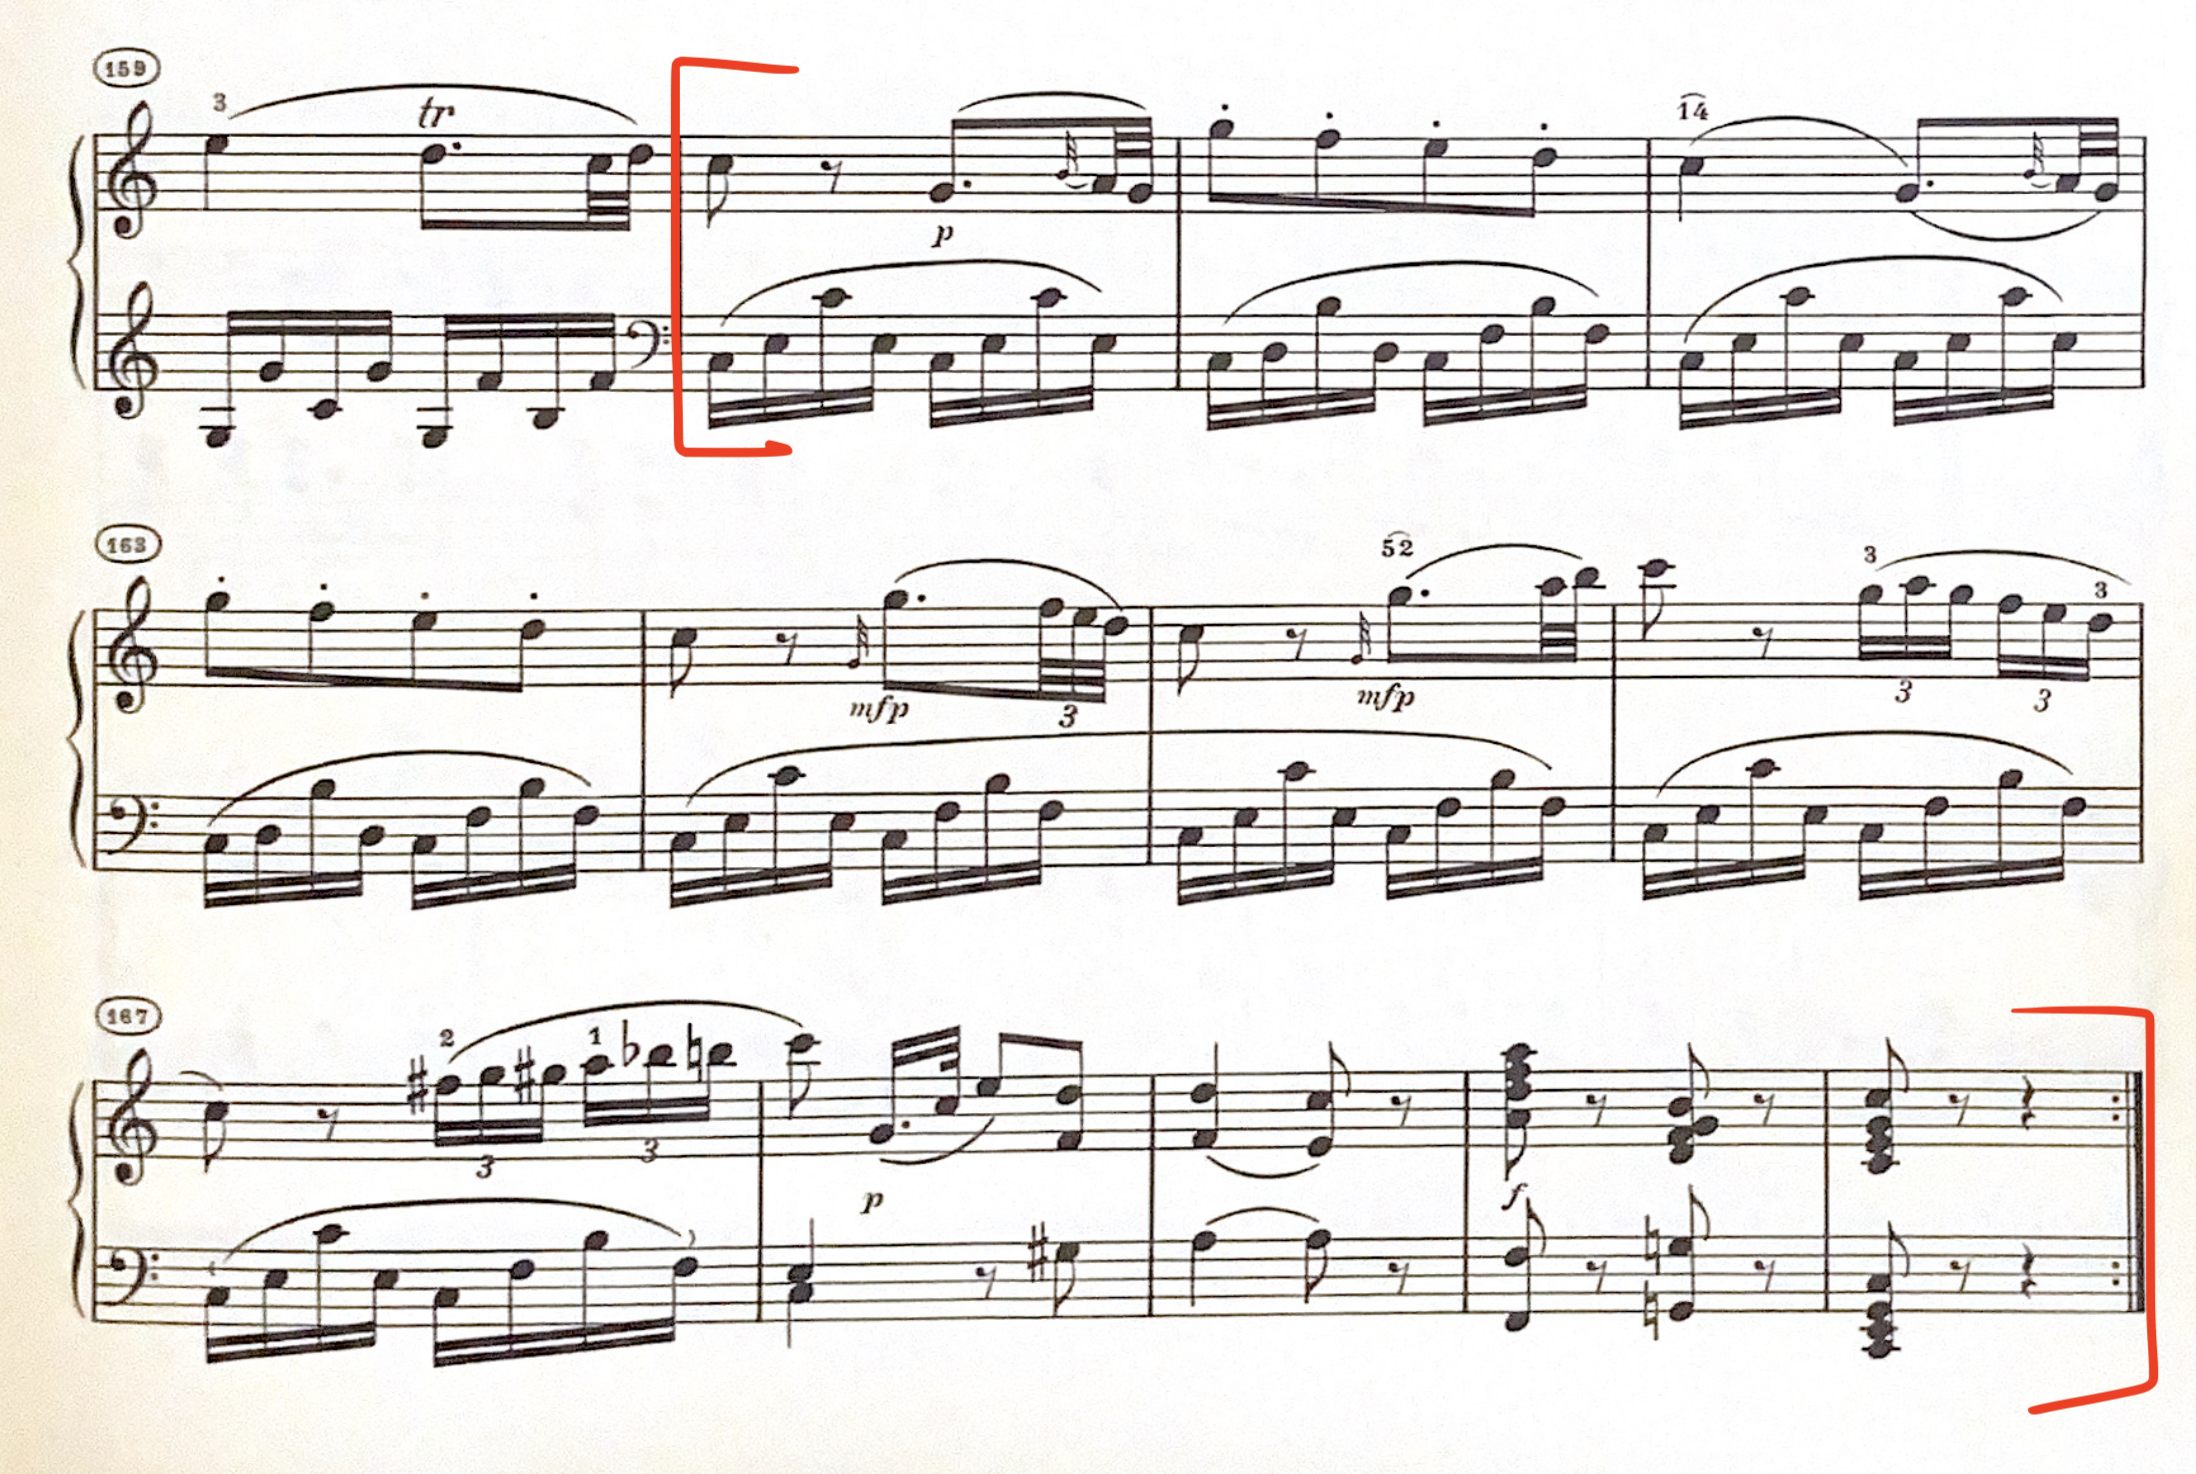
\includegraphics[width=\textwidth]{figures/mozart-third-movement-coda.png}
    \caption{Mozart's \textit{Piano Sonata in C Major}, the coda of the third movement}
    \label{fig:mozart-third-movement-coda}
\end{figure}
